%==============================================================================
% Document header
%==============================================================================
\documentclass[a4paper,11pt]{article}
\usepackage[pdfborder= 0 0 0 1]{hyperref}
\usepackage{graphicx}
\usepackage{multirow}

\usepackage{color}

\usepackage[toc,page]{appendix}

% Header and footer customization
\usepackage{fancyhdr}
\setlength{\headheight}{15.2pt}
\pagestyle{fancy}
\fancyhead[L]{\nouppercase{\leftmark}}
\fancyhead[R]{} 
\renewcommand{\footrulewidth}{0.4pt}

%==============================================================================
% Start of document
%==============================================================================
\begin{document}

%------------------------------------------------------------------------------
% Title
%------------------------------------------------------------------------------
\begin{titlepage}

\vspace*{3cm}

\noindent{\LARGE \textbf{I$^2$C Slave Core}}

\noindent \rule{\textwidth}{.1cm}

\hfill\today

\vspace*{3cm}

\begin{figure}[h]
  
\includegraphics[height=3cm]{fig/cern-logo}
  \hfill
  
\includegraphics[height=3cm]{fig/ohwr-logo}
\end{figure}

\vfill

\noindent {\Large \textbf{Theodor-Adrian Stana (CERN/BE-CO-HT)}}

\noindent \rule{\textwidth}{.05cm}

\end{titlepage}


%------------------------------------------------------------------------------
% Revision history
%------------------------------------------------------------------------------
\thispagestyle{empty}
\section*{Revision history}

\centerline
{
  \begin{tabular}{l c p{.6\textwidth}}
  \hline
  \multicolumn{1}{c}{\textbf{Date}} & \multicolumn{1}{c}{\textbf{Version}} & \multicolumn{1}{c}{\textbf{Change}} \\
  \hline
  23-11-2013 & 0.1 & First draft \\
  \hline
  \end{tabular}
}

\pagebreak
\pagenumbering{roman}
\setcounter{page}{1}
\tableofcontents

%------------------------------------------------------------------------------
% List of figs, tables, abbrevs
%------------------------------------------------------------------------------
\pagebreak
\listoffigures
\listoftables

\section*{List of Abbreviations}
\begin{tabular}{l l}
FSM & Finite State Machine \\
\end{tabular}

\pagebreak
\pagenumbering{arabic}
\setcounter{page}{1}

%==============================================================================
% SEC: Intro
%==============================================================================
\section{Introduction}
\label{sec:intro}

The Finite State Machine (FSM) Watchdog Timer component (\textit{gc\_fsm\_watchdog})
is a simple component that can be used to reset an FSM in case it spends too much
time outside the state machine's IDLE state. The component asserts its output signal
when the watchdog reaches a user-selected value. This output can then be used
in the HDL code to reset the FSM.

%==============================================================================
% SEC: Instantiation
%==============================================================================
\section{Instantiation}
\label{sec:instantiation}

The ports of the \textit{gc\_fsm\_watchdog} module are shown in Table~\ref{tbl:ports}.

\begin{table}[h]
  \caption{Ports of \textit{vbcp\_wb} module}
  \label{tbl:ports}
  \centerline
  {
    \begin{tabular}{l c p{.6\textwidth}}
    \hline
    \multicolumn{1}{c}{\textbf{Port}} & \textbf{Size} & \multicolumn{1}{c}{\textbf{Description}} \\
    \hline
    clk\_i      & 1 & Clock input \\
    rst\_n\_i   & 1 & Active-low reset input \\
    wdt\_rst\_i & 1 & Active-high reset input from the FSM to the watchdog timer \newline
                      Synchronous to \textit{clk\_i}\\
    fsm\_rst\_o & 1 & Active-high reset output from the watchdog timer to the FSM \newline
                      Synchronous to \textit{clk\_i}\\ \\
    \hline
    \end{tabular}
  }
\end{table}

Figure~\ref{fig:conn} shows how the \textit{gc\_fsm\_watchdog} module can be connected
to an FSM in a design. The clock (\textit{clk\_i}) and active-low reset (\textit{rst\_n\_i})
input ports should be connected to the master reset lines in the design. The signal connected
to the active-high input reset port (\textit{wdt\_rst\_i}) should be asserted by the FSM when
it is in its IDLE state. The reset output to the FSM (\textit{fsm\_rst\_o}) should be
ORed together with the active-low master reset input and connected to the reset input
of the FSM.

\begin{figure}[h]
  \centerline{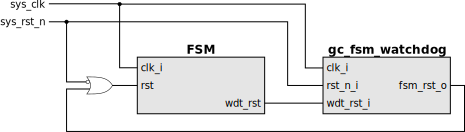
\includegraphics[width=.9\textwidth]{fig/conn}}
  \caption{Connecting the \textit{gc\_fsm\_watchdog} module to an FSM}
  \label{fig:conn}
\end{figure}

Examples of how to connect to the \textit{gc\_fsm\_watchdog} module are given in
Appendix~\ref{app:instantiation}.

%==============================================================================
% SEC: Instantiation
%==============================================================================
\section{Implementation}
\label{sec:implem}

The watchdog timer is implemented as a simple up-counter which asserts the
\textit{fsm\_rst\_o} output when the maximum value of \textit{g\_wdt\_max} is
reached. The counter is reset by either the active-low (system) reset and the
active-high (FSM) reset. A diagram of the block is shown in Figure~\ref{fig:implem}.

\begin{figure}[h]
  \centerline{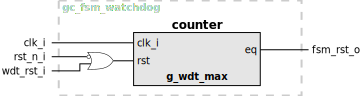
\includegraphics[width=\textwidth]{fig/implem}}
  \caption{Diagram of the FSM watchdog module}
  \label{fig:implem}
\end{figure}

%==============================================================================
% APPENDICES
%==============================================================================
\pagebreak
\begin{appendices}

\section{Example instantiation}
\label{app:instantiation}

\subsection{VHDL}

\begin{verbatim}
p_proc : process (sys_clk)
begin
  if rising_edge(sys_clk) then
    if (sys_rst_n = '0') or (rst_fr_wdt = '1') then
      state <= IDLE;
    else
      case state is
        when IDLE =>
          wdt_rst <= '1';
          if (trigger = '1') then
            wdt_rst <= '0';
            state   <= NEXT_STATE;
          end if;
        when NEXT_STATE =>
          -- ...
      end case;
    end if;
  end if;
end process p_proc;

cmp_fsm_watchdog : gc_fsm_watchdog
  generic map
  (
    -- FSM should return to IDLE within 256 clk_i cycles
    g_wdt_max => 256
  )
  port map
  (
    clk_i     => sys_clk;
    rst_n_i   => sys_rst_n;
    wdt_rst_i => wdt_rst;
    fsm_rst_o => fsm_rst;
  );
\end{verbatim}

\pagebreak
\subsection{Verilog}

\begin{verbatim}
always @(posedge sys_clk)
  begin
    if (!rst_n_i) or (rst_fr_wdt) then
      state <= IDLE;
    else
    begin
      case (state)
        IDLE:
          begin
            wdt_rst <= 1'b1;
            if (trigger = '1') then
            begin
              wdt_rst <= 1'b0;
              state   <= NEXT_STATE;
            end
          end
          
        NEXT_STATE:
          begin
            // ...
          end
      endcase
    end
  end
  
gc_fsm_watchdog cmp_gc_fsm_watchdog (
  .clk_i     (sys_clk),
  .rst_n_i   (sys_rst_n),
  .wdt_rst_i (wdt_rst),
  .fsm_rst_o (rst_fr_wdt)
)
\end{verbatim}

\end{appendices}


%==============================================================================
% Bibliography
%==============================================================================
%\pagebreak
%\bibliographystyle{ieeetr}
%\bibliography{gc_fsm_watchdog}

\end{document}